\chapter{Charting Deep-Sea Hydrothermal Plumes in the Field}
\label{chap:field_results}

With autonomy tools in hand that support a realistic \emph{deployment-by-deployment} field operations scenario, the question remains on their efficacy while in the field. Continuing with a focus on the charting of deep-sea hydrothermal plumes, this chapter discusses the engineering practicalities of arriving to a sensor model from scientific field data suitable for \PHUMES, using \PHORTEX to plan AUV \Sentry missions, and qualitatively comparing the performance of these trajectories with science-team designed dives. We also examine how a trained \PHUMES representation, and the data collected at sea, lend themselves to different downstream scientific inquiries. Research presented in this chapter is adapted from~\cite{preston2022physically}.

\section{Introduction}
As presented in \cref{chap:phortex}, \PHORTEX (with \PHUMES embedded), is an autonomy system designed to uncover the dynamics model of spatiotemporal distributions from sparse observations, and leverage that dynamics model to plan strategically useful trajectories for AUV \Sentry to execute during non-adaptive multi-hour dives. In this formulation, two key assumptions made was access to a binary measurement of the presence or absence of plume-derived fluids, and availability of sensors of opportunity to define or constrain the physically-informed layer of the \PHUMES model. 

Access to a binary measurement has been generally assumed in vent-hunting or source-seeking literature\autocite{tian2014behavior,saigol2009information,jakuba2007stochastic} as a means for ultimately detecting, with confidence, the buoyant stem of a plume expression, which is informative of the vent location. As established in \cref{chap:afar}, there is no ``plume detector'' on an AUV, and so this measurement must be approximated from continuous measurements from multiple science sensors. This lack of exact sensing is due to the variable values of temperature, chemistry, and particulate matter that persist within a plume structure. In the buoyant stem of a plume, positive temperature anomalies may be several degrees warmer compared to ambient seawater; however in the neutrally-buoyant plume layer, these anomalies may be on the scale of sensor noise (only a few hundredths of a degree). Chemistry anomalies may persist longer within a plume, but are subject to unknown and variable rates of microbial digestion or chemical reaction with the environment. Moreover, some chemical signatures may not specifically fingerprint hydrothermal anomalies, and could be equally indicative of other water-mass mixing events in the deep ocean. Finally, some oceanographic properties (e.g., temperature) vary in the water column as a function of depth, and so data must be detrended with respect to position in the water column. Taken together, the environmental complexity requires developing a sensing strategy that can fuse observations from multiple science sensors onboard AUV \Sentry into a data product that indicates whether the robot encountered hydrothermal plume fluids.

Separately, binary measurements alone are not easily informative of other types of structure useful for formulating the \PHUMES predictive model. Opportunistic sensor deployments, or leveraging the continuous value of strategic onboard sensors, may be one key way of alleviating the burden on the binary detections alone. Opportunistic sensor deployments are those science party activities which yield data products that can be widely applicable across projects. For instance, deployment of a CTD Rosette is a common practice at sea, and the vertical water column profiles that can be collected from these deployments can be directly useful in \PHUMES to set reference stratification curves utilized by the buoyancy flux computation within the scientifically-informed layer. Identifying, processing, and incorporating these types of measurements requires close collaboration with the science party (and some creativity), and here we discuss how we leveraged remotely operative vehicle (ROV) \emph{JASON} observations, a CTD Rosette, and a bottom-mounted tiltmeter within \PHUMES during field operations.

Finally, the ultimate goal of utilizing \PHORTEX is to collect observations that are useful for downstream science tasks. Here, we investigate the utility of \PHUMES as a scientific data tool for uncovering vent characteristics and corresponding estimates for energy flux, in addition to the explanatory power of \PHUMES for the distribution of plume-derived fluids in the basin. The use of idealized models such as~\cite{morton1956turbulent} or~\cite{speer1989model} for estimating heat (and other energy) fluxes from collected observations at a vent source are common in scientific publications in hydrothermalism\autocite{barreyre2012structure,wilson1996hydrothermal,mittelstaedt2012quantifying,baker1993method,ramondenc2006first}. While useful, these models fail to consider the impact of crossflow on the observable characteristics of a plume from water column data.



\paragraph{Contributions}
We demonstrate \PHORTEX with \PHUMES in field trials for hydrothermal plume charting with AUV \Sentry. In so doing, we present a method of processing real \emph{in situ} observations taken by instruments on \Sentry into a data product which can be used to indicate whether a particular observation is plume fluid or ambient seawater. We also discuss the practicalities of using external sensing equipment available during the field trial to benefit the \PHUMES formulation. Additionally, through this trial we demonstrate the first iterative offline planning technique for plume charting with deep-sea capable vehicles, illustrating a novel capability for these assets for future research expeditions and putting over 75\% of known vent fields\autocite{beaulieu2013authoritative} in reach for strategic charting and surveying. In study of the field trial results, we investigate the quality of the scientific observations that are collected for several downstream scientific queries, including estimating energy flux and vent characteristics, and uncovering the structure of the neutrally-buoyant layer of a plume.

\section{Methods}
\label{sec:field_methods}

\subsection{Plume Detection: Treatment of Robotic Science Sensors}
\label{sec:sensor_models}
We elect to process the heterogeneous sensor stream into a binary measurement stream, drawing on the work in \autocite{jakuba2007stochastic}, to indicate whether \Sentry was in a plume or in background seawater\footnote{Access to a binary measurement for plume hunting has long been assumed in related work e.g.,  \autocite{tian2014behavior,saigol2009information}}. In our study, we use a conductivity probe (salinity), temperature probe (temperature), oxidation-reduction potential (ORP) instrument (relative ``reactivity'' of water), optical backscatter (OBS) instrument (turbidity), optode (oxygen), and experimental spectroscopic instruments Pythia \autocite{michel2022gas,Harb:12} and SAGE \autocite{kapit2021dissolved,kapit2021measurement} (dissolved methane) to compute a binary measurement. Sensors are internally logged at variable rates, but interpolated and sub-sampled to a fixed 1 Hz frequency with a shared clock time for the purposes of directly comparing the instruments. Each of these sensors has its own physical characteristics and response to the chemistry of plume water. For example, ORP exhibits a large negative spike when first encountering plume water followed by a slow hysteresis back to a nominal values. Measurements of salinity, temperature, and oxygen are expected to be influenced not only by plume water, but background physical mixing in the ocean; turbidity, ORP, and methane are signals strongly associated with hydrothermalism because they are not persistent in background seawater. To account for the different ways in which sensors respond to plume waters, each sensor is processed individually to detect plume masses in each stream (see \cref{tab:sentry_instruments}). Weights are assigned to each sensor based on their individual reliability for identifying plume water, as determined by the science party and consulted experts in preparation for the research expedition. Observations are then classified as plume water or background water using corroboration across sensors: weighted detections for each sensor are summed together and we use a detection threshold to identify an observation as plume or background. A total corroboration score of 4 or more was used to classify an observation as plume. An example of this sensor applied to real \Sentry detections is shown in \cref{fig:detection_example}.

\begin{table}[h!]
    \centering
    \begin{tabular}{c|c|c}
        Quantity & Positive Plume Detection Criteria & Weight  \\
        \hline
        Salinity & Detrended practical salinity outside 3 standard deviations of the entire time series & 1 \\
        Temperature & Detrended temperatures above the 75th percentile of entire time series & 2 \\
        ORP & Detections less than -0.005 & 2 \\
        OBS & Optical attenuation above the 75th percentile of entire time series & 2 \\
        Oxygen & Detrended concentrations outside one-hour rolling computation of 3 standard deviations & 1 \\
        Methane & Normalized concentration above 0.3 & 2
    \end{tabular}
    \caption{\textbf{Instruments on AUV \Sentry and the criteria used to identify plume fluids for each instrument.} The weight is used to indicate relative trustworthiness of a plume detection for each sensor, and is used in a corroboration scheme that sums detections across sensors in order to make a final determination on whether an observation location contained a parcel of plume fluid or consisted of background seawater. Detrended data removes depth-related cross-sensitivity from the measurements; for example, temperature is stratified in the deep ocean, so to ignore the impacts of depth changes in the data stream, those effects are removed by ``detrending'' the data stream.}
    \label{tab:sentry_instruments}
\end{table}

\begin{figure} [h]
    \centering
    \includegraphics[width=0.45\columnwidth]{figures/binary_example_time.png}
    \hspace{.1in}
    \includegraphics[width=0.45\columnwidth]{figures/binary_example_detections.png}
    \caption{\textbf{Example time series (left) and associated detections (right) over the AUV \Sentry sensor suite.} Oxygen, temperature, and salinity measurements are detrended using a linear transformation fit to depth vs. value plots. The time series demonstrates two types of plume detections. The first are ``obvious detections'' in which most sensors register strong anomalies (this happened twice toward the end of the deployment) and are most strongly associated with buoyant-stem derived fluids. The second are ``persistent-plume detections'' in which the robot traverses through water that is slightly more turbid, warm, or chemical-rich than background water over potentially long horizons (this happened early in the deployment and in the middle). Such detections are most strongly associated with neutrally-buoyant layers. The conservative corroboration detector successfully identifies both forms of plume water.}
    \label{fig:detection_example}
\end{figure}

% This approach for processing complex sensor observations into binary plume detections was initially developed by \autocite{jakuba2007stochastic}; our method is an adaptation of the process using recommendations in this previous work and in consultation with the science team we were directly collaborating with for this study. 
The result of our sensor model is to convert multiple, time-stamped sensor observations $s_{t, i} \in \R, \, i = 1, \dots, S$ to a time-stamped binary plume-detection $z_{p, t} \in \{0, 1\}$. These binary plume detections are then used to update our plume model and plan robot trajectories, as described in the following sections. The accuracy of this sensor model is currently uncharacterized, as there is no available ground truth in a field setting by which to verify the assigned classifications. Qualitatively, the classifications were reviewed by the science team and verified for their alignment with expert opinions on which label to assign.


%%%%%%%%%%%%%%%%%%%
% External Sensing 
%%%%%%%%%%%%%%%%%%
\subsection{External Sensing: Leveraging All Available Information}
\label{sec:external_current}
We deployed several sensing packages during the research cruise to collect relevant information about the state of temporally evolving crossflow $\x_c$ and ambient seawater properties. We leverage these external measurements within our \PHUMES instance in two ways. First, we characterize the background seawater stratification near a target site using a ship-board rosette\footnote{A rosette is often a metal frame on which oceanographic sensors and a carousel of water sampling containers are mounted. It is attached to a ship via a cable, and can be lowered and raised via a winch in vertical transects of the water column, or can be towed by a moving ship horizontally through the water column.} which takes vertical profiles of the water column. The empirical stratification function for Guaymas Basin is used within the physically-informed layer of \PHUMES and treated as a constant throughout the expedition. Second, we learn the crossflow transition function $T_c$. Critically there was no sensor on \Sentry during our expedition that could be used to measure the \emph{in situ} current magnitude and heading. While it may be possible to estimate $T_c$ solely from the binary observations of the plume, access to an external bottom-mounted tiltmeter on the seafloor during this expedition significantly relieved the burden of this inference process. These auxiliary sensors are introduced and discussed in detail in \cref{sec:field_results}. 

% For the former (1), measurements from a temperature and salinity sensor mounted to a ship-board rosette were used to define the depth-dependent density, temperature, and salinity stratification curves of the field site (Guaymas Basin) water column. The stratification curve is a function that describes the changes in density over depth in the ocean, and has implications for how a hydrothermal plume will interact with background seawater. 

% We learn $T_c$ (or, more precisely, the function $h$ by which $T_c$ is defined) by fitting a Gaussian process (GP) with composite radial-basis-function and periodic kernel functions to point observations of crossflow magnitude and heading observed by the tiltmeter. Approximately 3 days of observations were available for training. Crossflow parameters $\x_c$ in $\Ss$ were set with the expected mean of the trained GP. At present, a crossflow sensor is in development for \Sentry using existing acoustic technology onboard the robot; in such a configuration, estimating $T_c$ could be done simultaneously with the plume-charting task.

\subsection{At Sea Operations}
\PHORTEX was used to enable deployment-by-deployment autonomy during field operations with AUV \emph{Sentry} that fit within the typical workflow of operations at sea (\cref{fig:at_sea_ops}). Functionally, the trajectories planned with \PHORTEX were provided to the \Sentry engineering team for extensive safety validation prior to each deployment. If approved by the \Sentry team, the chief scientist, and captain of the vessel, the trajectories were downloaded into the \Sentry mission planning software as static waypoints. This confirmation process required a lead time of approximately 6 hrs before a scheduled deployment, and 12-18 hrs were available between deployments to mechanically service \Sentry and recharge batteries. The ability of \PHORTEX to produce viable trajectories from data within the first 6 hrs that \Sentry was on-deck following a recovery was critical for keeping this strict timeline. Given the long lead time between trajectory design and \Sentry deployment, there were many opportunities for the time of a deployment to change due to e.g., developments in weather, or other science/technology priorities. To be robust to these changes, we provided deployment plans that started several hours before and several hours after a given deployment time, and the \Sentry team truncated the plan at the appropriate points once a deployment time was known with certainty.

\begin{figure}[h!]
    \centering
    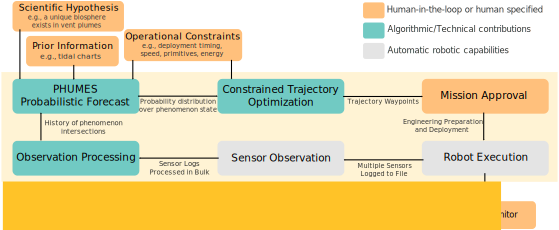
\includegraphics[width=0.9\columnwidth]{figures/deployment_loop.png}
    \caption{\textbf{The operational implementation of \PHORTEX at sea.} Integration of scientific knowledge, prior information, auxiliary sensor information, and operational constraints was done at the initialization of the \PHORTEX deployment-by-deployment loop. Every trajectory generated by \PHORTEX was checked by AUV \Sentry engineers and the science team before execution. \Sentry status was monitored with an external acoustic tracking system that monitored vehicle location, power, and performance while in acoustic range of the ship. Upon returning to deck, all science sensor observations were downloaded in bulk from the vehicle, and then ingested via our \PHORTEX system.}
    \label{fig:at_sea_ops}
\end{figure}

% \PHORTEX produces a chained trajectory object, informed by the probabilistic plume forecast. A set of extensive safety checks and human validation steps are subsequently performed on the planned trajectory. The ship is then moved to the deployment point, which is determined by the ship captain based on the planned trajectory and the constraints of other ship operations. \emph{Sentry} was deployed and executed the chained trajectory, collecting scientific sensor observations. Deployments generally lasted 17-20 hours due to battery limitations, after which \emph{Sentry} is recovered by the ship. After recovery, the data collected by \emph{Sentry} is downloaded and used to update \PHUMES as in \cref{sec:phumes}. The updated belief from \PHUMES is then used to plan a new chained trajectory, as described in \cref{sec:to}. These belief update and planning steps can take place over several hours ($<$10 hrs) while the AUV batteries are recharged.

\section{Description of Field Site}
In November 2021, a research cruise aboard the research vessel (R/V) \emph{Revelle} was conducted at the Northern Guaymas Basin in the Gulf of California to study a recently discovered hydrothermal ridge \autocite{soule2018exploration, geilert2018formation}. The research cruise had several objectives: test novel \emph{in situ} instruments to measure dissolved methane, test novel \emph{in situ} instruments to measure the carbonate cycle, map the heat distribution in shallow sediments above hydrothermal sills, collect specimens of tubeworms, and collect biological samples of microbiota in hydrothermal plume-fluids to re-construct the structure of a plume microbiome. It is typical that research cruises have several science teams working together under an appointed chief scientist to maximize the use of ship assets while at sea. To assist in operations, AUV \Sentry, remotely-operated vehicle (ROV) \emph{JASON}, and standard oceanographic equipment were available. The deployment of \PHORTEX on the cruise for \Sentry operations was coupled with objectives to test \emph{in situ} instruments and collect microbiota samples. For both of these tasks, charting different regions within a plume was important to test the capabilities of the novel instruments and collect biological samples from a diversity of plume-conditions.

% \begin{figure}[h!]
%     \centering
%     \includegraphics[width=\columnwidth]{figures/transect_overview.jpg}
%     \caption{\td{this is just a placeholder! An adjusted version of this with better bathy + pictures of the vent from the seafloor + just focused on Sentry lawnmowers will be put here instead. Maps will be preserved for context setting} Located in the northern Guaymas Basin in the Gulf of California, a hydrothermal ridge served as a target for charting mid-water plume structures by AUV \emph{Sentry}.}
%     \label{fig:bathy_vent}
% \end{figure}

\subsection{Site Description and General Conditions}
The main site for the study conducted by AUV \Sentry using \PHORTEX was a hydrothermal ridge located in the northern Guaymas Basin, approximately \SI{1850}{\meter} underwater and at the edge of an additionally \SI{300}{\meter} deeper graben (a valley with steep sides) (\cref{fig:site}). The ridge is approximately \SI{600}{\meter} long and features several tall sulfide structures 45-\SI{75}{\meter} in height with active smoking along their bodies. A smoking ``chimney'' at the northernmost point of the ridge was targeted for plume-charting. The chimney vent was composed of a cluster of tens of small orifices ($<$\SI{0.1}{\meter} diameter) that created an approximately \SI{1.5}{\meter} diameter chimney base. The fluid produced was thick with particulate matter and measured with a temperature wand on ROV \emph{JASON} to be \SI{340}{\celsius} at the source. Fluids ventilated rapidly at approximately \SI{0.7}{\meter\per\second} (as measured by video equipment) and were rich in dissolved methane. In contrast, the ambient seawater was methane-poor, considerably less turbid, and cold at \SI{4}{\celsius}. As vent fluids rise and form a plume at this site, the ambient water is mixed (entrained) at an unknown rate, and advected by mild deep-water currents. Under these conditions, plume expressions could be transported several hundred meters from a known source, and would be expected to rise over \SI{200}{\meter} in the water column. In scientific work following this expedition, plume fluids were identified up to \SI{7}{\kilo\meter} away from known venting sites \autocite{preston2022discovering}. 

\begin{figure}[h!]
    \centering
    \includegraphics[width=\columnwidth]{figures/site_summary.png}
    \caption{\textbf{Study site in the Guaymas Basin, Gulf of California.} The inset map is bathymetric data collected by AUV \Sentry during this expedition and shows the approximately \SI{600}{\meter} long ridge in yellow. The red star marks the chimney that was of particular study in this article. Pictures A-D show imagery from the ridge and chimney site. A-C show various forms of plume-producing vents located at the chimney and D shows an example of the macrofauna covering the structures along the ridge.}
    \label{fig:site}
\end{figure}

\subsection{Available Oceanographic Instrumentation}
\label{sec:aux_sensors}
Observations from external sensors, summarized in \cref{tab:ext_sensors} and visualized in \cref{fig:ext_sensors}, were incorporated into the initial conditions, temporal functions, and seawater properties that define the analytical model in \PHUMES as described in \cref{sec:external_current}. Vent characteristics (i.e., vent area, vent fluid velocity, fluid temperature at the vent) were measured by ROV \emph{JASON} during other field operations in the expedition. \emph{JASON} carried a camera system and temperature wand. Measuring temperature with an ROV is precise, and so we directly use the observation of temperature by \emph{JASON}, \SI{340}{\celsius}, as the initial condition for vent fluid temperature in the \PHUMES model trained with at-sea data. Vent area and vent fluid velocity are measured with cameras onboard ROV \emph{JASON}. Using a \SI{10}{\centi\meter} spaced set of laser points that \emph{JASON} can toggle on and off \emph{in situ}, the vent area is extrapolated from an estimate of vent diameter from pixel-to-distance conversion in still images. Using this method, an area of approximately \SI{1.7}{\meter\square} was estimated, and used to center a uniform distribution over vent area to be updated with \PHUMES. Vent exit velocity was estimated by applying particle imaging velocimetry (PIV) \autocite{zhang2019time} to 4K video of the turbid fluids at the vent. PIV methods track turbulent parcels that have high cross-correlation values between frames of a video. By tracking many parcels over several frames, PIV yields a vector field of velocity estimates that can be averaged to establish a mean estimate for a region. Using \verb|PIVLab|, an open-source \verb|MATLAB| library, we estimated a fluid exit velocity of \SI{0.7}{\meter\per\second}, and similarly use this as the center of a uniform prior placed on exit velocity for \PHUMES to update.

\begin{table}[h!]
    \centering
    \begin{tabular}{c|c|c|c}
        Platform & Instrument & Data Product & \PHUMES Incorporation \\
        \hline
        ROV \emph{JASON} & Camera & Vent Area &Informs prior over vent area \\
        ROV \emph{JASON} & Camera & Fluid Exit Velocity & Informs prior over fluid exit velocity \\
        ROV \emph{JASON} & Temperature wand & Vent Temperature  & Sets temperature initial condition \\
        Rosette & CTD probe & Water Column Stratification & References for analytical model \\
        Tiltmeter & Accelerometer & Current magnitude, heading & Use trained GP in forecast sampling \\
    \end{tabular}
    \caption{\textbf{Summary of auxiliary data.} External equipment and opportunistic data available from other operations during the field expedition that was used to inform the \PHUMES model within \PHORTEX used for at-sea trials.}
    \label{tab:ext_sensors}
\end{table}

In addition to \emph{JASON}, vertical profiles from a rosette of ambient seawater background salinity and temperature were available. As reference density and density stratification for a body of water are parameters of the analytical model (in order to compute buoyancy flux for the hydrothermal fluid), these profiles were used directly for this purpose. As the data had small amounts of noise, we fit simple Gaussian Process (GP) models with radial-basis function (RBF) kernels to each of temperature and salinity from a conductivity-temperature-depth (CTD) probe on the platform using \verb|GPytorch| (100 iterations, learning rate 0.1), and use the trained mean function within \PHUMES.

Finally, a tiltmeter (an instrument that is fixed to the seafloor on one end, and is allowed to tilt under the effects of crossflow) was available and deployed on the seafloor for three days during the cruise. Data collected from this instrument can be used to compute crossflow magnitude and heading. We observed a maximum crossflow magnitude of approximately \SI{0.1}{\meter\per\second}, and both magnitude and heading appeared to be semi-cyclic, following a pattern established by tidal charts produced by Centro de Investigaci\'on Cient\'ifica y de Educaci\'on Superior de Ensenada (CISESE) for the time period of the expedition\footnote{Charts available from: \url{www.predmar.cicese.mx/calendarios}}. Time-varying currents of magnitudes between 0.1-\SI{0.5}{\meter\per\second} sweeping from the northwest to southwest were previously reported in \autocite{scholz2019shelf}, corroborating our observations. We similarly trained a GP with RBF kernel for each of current magnitude and heading using \verb|GPytorch| (magnitude model: 100 training iterations, learning rate 0.5; heading model: 200 training iterations, learning rate 0.1), and used the trained GP within the sampling framework for \PHUMES to generate forecasts. 

\begin{figure}[h!]
    \centering
    \includegraphics[width=1\columnwidth]{figures/external_sensors.png}
    \caption{\textbf{Auxiliary data products used in \PHUMES.} External equipment (ROV \emph{JASON}, tiltmeter, and rosette) provided opportunistic data products during the field expedition that were incorporated into \PHUMES. The ROV \emph{JASON} was used to determine prior estimates for the plume source parameters. The rosette collected vertical temperature and salinity profiles which are used to compute stratification in the basin. A GP is trained over the data, and the mean is visualized in the lower right panel. The tiltmeter records data of current magnitude and heading; a GP was trained over both functions and is visualized in the lower left panel. Heading is reported in compass-rose orientation.}
    \label{fig:ext_sensors}
\end{figure}




\section{Performance of \PHORTEX}
\label{sec:phortex_performance}
Four deployments of AUV \Sentry were available to study the hydrothermal site. These deployments represent a planning spectrum, from fully human-designed surveys to fully \PHORTEX designed. We label the four deployments as follows:
\begin{itemize}
    \item \textbf{Dive H-Multi}: human designed, multi-task survey. This was the first deployment of \Sentry and the survey was designed to both attempt to find plume fluids and to bathymetrically map the local basin area (the map of which would be used as part of the safety check protocol for future deployments). This dive is representative of a standard nested strategy, in which progressively more targeted (finer resolution) surveys are used to study areas of interest. The dive was designed by a human expert who only had access to the approximate location of the target vent. The deployment lasted 21.3 hrs and collected 76,604 observations total.
    \item \textbf{Dive H-Plume}: human designed, plume-charting survey. This was the second deployment of \Sentry and the survey was hand-designed by the science party onboard the vessel to find and sample plume fluids. The science party had access to the performance of \Sentry in Dive H-Multi. The strategy was to sweep the basin above areas with known hydrothermal vents, and fly out into the basin in the direction that the plume fluids would be expected to advect. The deployment lasted 21 hrs and collected 75,430 observations total.
    \item \textbf{Dive HP-Plume}: hybrid human and \PHORTEX plume-charting survey. This was the third deployment of \Sentry and the survey consisted of trajectories designed by \PHORTEX trained by observations collected only in Dive H-Multi. Two of the trajectory primitives designed by \PHORTEX were replaced by ``naive'' lawnmowers placed over the known vent at two different times in the deployment. The deployment lasted 22.2 hrs and collected 79,792 observations total. Of these, 8.2 hrs and 29,438 observations were collected via the naive strategy.
    \item \textbf{Dive P-Plume}: \PHORTEX plume-charting survey. This was the fourth and last deployment of \Sentry. The survey was fully designed by \PHORTEX using observations only from Dive H-Multi, several days prior to this dive. The deployment lasted 9.9 hrs and collected 35,755 observations total. This deployment is notably much shorter than the other deployments due to increasing time constraints as the expedition was coming to a close. This deployment also used \Sentry in a ``depth-hold'' mode: whereas in all other dives \Sentry's depth followed the basin terrain, in this experiment the robot held an absolute depth.
\end{itemize}

Using the metrics introduced in \cref{sec:eval_metrics}, we evaluate each of the four dives executed at sea to chart the space-time dynamics of a real hydrothermal plume as presented in \cref{tab:field_results} and visualized in \cref{fig:field_results}. Each dive took place at different times in the tidal cycle, on different days, and often at different altitudes in the water column, and thus the total plume samples available to collect during each dive is variable. With this in mind, we present and evaluate each dive quantitatively, and additionally qualitatively examine each as a case study for how different sampling paradigms perform in the real-world. There is no ground-truth available for the deep sea plume-charting problem; we evaluate each \Sentry dive assuming that the binary detections produced by the method in \cref{sec:sensor_models} are honest representations of the presence or absence of hydrothermally-derived fluids in the basin. 

The results of the field deployment in \cref{tab:field_results} demonstrate that \PHORTEX performs comparably to science expert-designed trajectories in the proportion of samples that are collected during dives, and importantly improves upon the spatial utilization (increasing both the range of the most distal plume detection and effectively utilizing of the entire explored range). This is most evident in the HP-Plume dive, in which the human designed portion is a naive lawnmower placed ``on top'' of the vent; the \PHORTEX-designed trajectory collects samples over twice as far from the plume source. Absolute temporal utilization is similar to human surveys; however the distribution of detections within the temporal utilization windows is improved --- for human surveys, detections tend to be ``bunched'' to either the first half (as in H-Plume) or second half (as in H-Multi). We see this most sharply in HP-Plume, in which 90\% of positive detections collected by the human-designed survey occurred only in the second of the two lawnmowers, from hours 20-23. In contrast, \PHORTEX designed trajectories collected detections more uniformly over the entire dive.  \cref{fig:field_results} shows the qualitative structure of each dive and showcases the diversity in the resulting datasets.

% Evaluating the efficacy of human- and \PHORTEX-designed trajectories in charting the space-time dynamics of a real-world hydrothermal plume is challenging. Unlike the simulation experiments, there is no ground-truth plume chart available and evaluating the counterfactual --- if \PHORTEX had gone here instead, how many more observations of the plume would have been collected? if we had used a naive planner instead of \PHORTEX for this deployment, how many fewer observations of the plumes would we have?--- is not straightforward. Due to operational constraints and the value of ship time, using an entire deployment of \Sentry to implement a lower-performing baseline is prohibitively wasteful; each deployment attempts to make the best use of available data to accomplish the task of plume charting.  In the remainder of the section, we evaluate each \Sentry dive using the metrics introduced in \cref{sec:eval_metrics}, assuming that the binary detections produced by the method in \cref{sec:sensor_models} are ground-truth detections and non-detections. 

% We look at several key metrics for each deployment: proportion of positive plume observations, utilization of spatial extent, and utilization of temporal dive window. The first metric, proportion of positive plume observations, is simply the number of observations collected in a dive that were classified as in-plume by the binary sensor model we describe in \cref{sec:sensor_models}. The second metric attempts to show how spatially effective the design of the survey was by first showing the absolute range that positive detections were made as a measure of distance from the chimney vent location and second showing how that range fit with the overall design of the survey. For example, if detections were made up to 300 m away from the vent, but the robot traveled up to 1 km away, then the survey spent too much time outside of the detectable plume region and would not be as effective as a survey that only traveled 200 m away but stayed well within the detectable plume range. Finally, the last metric is a measure of how effective the survey was at \emph{staying in} or \emph{revisiting} a plume over time. Given the duration of these missions, it is important to use the entire mission window for the task at hand; moreover temporally ``diverse'' observations are of scientific interest generally. We report the proportion of dive hours with at least 10\% or more positive detections.



\begin{table}[h!]
    \centering
    \begin{tabular}{c|c|c|c|c|c}
        Dive & Duration & Total Obs. & Prop. In-Plume & Spatial Util. & Temporal Util.  \\
        \hline
        H-Multi & 21.3 hrs & 76,604 & 22.3\% & \SI{300}{\meter} (19\%) & 9-17,20-21 (52\%) \\
        H-Plume & 21 hrs & 75,430 & 10.9\% & \SI{900}{\meter} (64\%) & 2,5-8,10-11,15-16 (43\%) \\
        \hline
        HP-Plume & 22.2 hrs & 79,792 & 41.8\% & \SI{600}{\meter} (100\%) & 1-3,5,7,11-23 (81\%) \\
        HP-Plume (H) & 8.2 hrs & 29,438 & 42.3\% & \SI{250}{\meter} (100\%) & 5,7,20-23 (75\%) \\
        HP-Plume (P) & 14 hrs & 50,354 & 41.5\% & \SI{600}{\meter} (100\%) &  1-3,11-20 (93\%)\\
        \hline
        P-Plume & 9.9 hrs & 35,755 & 12.8\% & \SI{450}{\meter} (100\%) & 1,5,8,9 (40\%)
    \end{tabular}
    \caption{\textbf{Per-dive statistics for field trials of \PHORTEX.} The spatial utilization is reported as both the most distal plume detection (measured from the plume origin) and the ratio of the most distal plume detection over the farthest distance that the robot traveled from the plume origin. Temporal utilization shows both which hours contain at least 10\% positive plume detection and what fraction of the total deployment duration contained such detections. The deployment HP-Plume is broken further into human designed (H) and \PHORTEX designed (P) portions for direct comparison.}
    \label{tab:field_results}
\end{table}

\begin{figure}[h!]
    \centering
    \includegraphics[width=1.0\columnwidth]{figures/detections_data.png}
    \caption{\textbf{The four field dives of AUV \Sentry.} All data is plotted according to its detection identity (in-plume or seawater). The first column shows a top-view of the dive trajectories in polar coordinates, in which angle and radius is computed relative to the chimney coordinate of the vent of study. In the center column, the 3D path of the vehicle over the rendered bathymetric terrain is provided. All but Dive P-Plume were dives conducted in altitude-hold mode with \Sentry, and so the trajectories show obvious changes in elevation; in contrast Dive P-Plume was held in depth-hold mode, so most observations are gathered within a depth-plane. The final column shows a time series versus depth of the detections collected. In Dive HP-Plume the portions of the dive that were human-designed and \PHORTEX-designed are labeled with H and P, respectively. As can be seen in the Dive HP-Plume time series, the two human-designed trajectories have significantly different performance, despite being in locally similar regions of the spatial domain. }
    \label{fig:field_results}
\end{figure}

In this field deployment, we demonstrate that \PHORTEX is a useful and practical tool for plume-charting. The performance of trajectories designed with \PHORTEX are comparable to those designed by human experts with key improvements in spatial and temporal utilization. It is further worth highlighting that \PHORTEX was trained only on data collected during the first dive, H-Multi, and reasonable performance during P-Plume using week-old training data emphasizes the long-range forecasting ability of the approach. Practically, the automated nature of \PHORTEX operationally alleviates significant decision-making burden on a science team and the trajectory-design burden on the \Sentry team; the ability to ingest data from external sensors and previous \Sentry missions, and produce trajectories that can be seamlessly ingested by the safety checking system without human intervention is of considerable benefit in the field. Moreover, the intermediate products of \PHORTEX, such as \PHUMES forecasts, are useful for other tasks in field operations, such as deploying other instruments or prioritizing instrument deployment order based on temporal changes in the environment by virtue of yielding rich context easily interpretable by the science team. 

% Similarly, \PHORTEX is trained on significantly less data than what the human experts had access to throughout the cruise; this emphasizes the advantage of the model-based, data-aggregation approach in \PHUMES. 

\section{\PHUMES Validation with Basin Observations}
While there is no external ``ground-truth'' that we can use to evaluate the performance of \PHORTEX, we can compare the \PHUMES model trained on external and binary \Sentry observations with snapshots of the vertical distribution of turbidity near the hydrothermal ridge to get a sense for the utility of the \PHUMES model. After training, \PHUMES estimated the fluid exit velocity from the target chimney to be \SI{0.58}{\meter\per\second}, the vent area to be \SI{0.82}{\meter\squared}, and the vertical and horizontal mixing coefficients to be 0.15 and 0.19, respectively. Simulating these conditions with an initial vent temperature of \SI{340}{\celsius} and salinity of 34.908 PSU under a nominal crossflow of \SI{0.11}{\meter\per\second}, we compare the time-averaged plume height and width with the turbid intrusion that is observed in vertical casts of a shipboard rosette. The rosette was lowered and raised through the water column using a cable and winch on the ship; several vertical transects were collected over the course of the research cruise at the target autonomy site in addition to other sites throughout the basin. In \cref{fig:field_valid} we show two vertical transects, one conducted about \SI{100}{\meter} from a known vent, and one conducted \SI{600}{\meter} from the same vent. We see that within the model regions for predicted plume intrusions in the water column, strong turbid signals are observed in both vertical transects. This is indicative that the learned \PHUMES model is capable of uncovering the structure of the hydrothermal plume and lends confidence that the model is informative for planning sample trajectories that will intersect with plume fluids.

\begin{figure}[h!]
    \centering
    \includegraphics[width=1\columnwidth]{figures/field_validation.png}
    \caption{\textbf{Validation of \PHUMES model trained at sea.} We compare the nominal plume estimate from \PHUMES trained on at-sea data and \Sentry observations with vertical transects of turbidity from shipboard rosette. The plume envelope is the average plume estimated by \PHUMES for a nominal crossflow of \SI{0.12}{\meter\per\second}. Vertical red lines mark \SI{100}{\meter} and \SI{600}{\meter} laterally from the originating vent, for which vertical CTD casts were conducted. The region that the model estimates containing the lowest plume intrusion in the water column is highlighted on the turbidity transects. There is agreement between the model estimate and the transect data on the location of this turbid layer.} 
    \label{fig:field_valid}
\end{figure}

\section{Scientific Implications of Results}
\td{Would like to expand more on what the \PHUMES model tells us, some results on the buoyancy flux charts, and think about next steps}

\section{Discussion and Future Work}
\label{sec:future}
There is a significant desire for embodied intelligence and assistive decision-making in environmental exploration and expeditionary science. \PHORTEX fundamentally relies on human expertise to inform the scientific models used within \PHUMES, generate useful reward functions, set trajectory primitives, and for operational deployments on a robot while in the field. Relieving the burden on these human agents --- whether by creating aggregated data products or proposing multiple field missions with explanations --- could lead to significant gains in the short-term for expeditionary science tasks while robot technology matures. For instance, on the research cruise in this study, we created science-data displays for AUV \emph{Sentry} that graphed real-time science data reported at 0.02 Hz over an acoustic modem. While this is an extreme subset of the data, real-time reporting was sufficient for science experts to identify trends in robot performance with respect to the plume charting task. The capability of viewing real-time data, which to many academic and industrial roboticists may seem obvious or straightforward, is not yet pervasive or standard in the sciences or on state-of-the-art vessels and autonomous platforms. Research efforts on improving data infrastructure, data visualization, real-time signal processing, human decision-making, and supervised autonomy promise to be extremely impactful to the expeditionary sciences. 

\td{this paragraph needs edited because it shows up in the last chapter}
\PHORTEX is an autonomy system that has been demonstrated at-scale for a deployment-by-deployment mission to chart deep sea hydrothermal plumes, and showed quantitative gains over typical exploration strategies while also integrating into the operational ecosystem of a ship at sea. As technological advances in robot platforms increase for scientific contexts, advancing \PHORTEX for online settings and adapting multiagent strategies for deep-sea research are attractive next steps. For \PHUMES, improving upon the temporal expressivity of the model presented in this article, investigating pre-training opportunities with sophisticated simulators, and adapting state-of-the-art scientific machine learning techniques for a decision-making context, are areas of direct improvement that can be studied. The following sections discuss some of the key challenges in deploying \PHORTEX for hydrothermal plume charting, each of which may be avenues for future work. The section concludes with a discussion of how both \PHORTEX and \PHUMES, as modular frameworks, can serve as a methodological starting point for more general expeditionary science settings.


\paragraph{Compensating for Onboard Sensing Limitations of AUVs}
% comments on current inference and it being enabled by an external sensor
Leveraging sensing equipment external to a robot is well established for environmental studies in which satellite, fixed observatory, or historical observations are available. However, in many environments---subsea, subterreanean, forests---such observational equipment may not be available or needs to be independently deployed by a science team or by a robot explorer. The use of multiagent systems for environmental studies in spatiotemporal fields (e.g., \autocite{salam2019adaptive,li2014multi,luo2018adaptive,ouyang2014multi}) is particularly powerful, as robots can carry heterogeneous sensors and collect simultaneous observations in different spatial locations. As fleets of deep-sea capable robots are not generally within reach for the science community, in this article, we leveraged an external crossflow sensor deployed by the science team and other standard shipboard sensing equipment to compensate for information that would have been difficult (or impossible) to collect with AUV \Sentry otherwise. Without access to these external sensors, additional burdens would need to be placed on the environmental model and inference methods used for decision-making. 

\paragraph{Scientific Implications of the Collected Data}
Tens of thousands of \emph{in situ} observations were collected in the four field dives that were executed in this study. These data can be directly used in external scientific frameworks for investigating hydrothermalism expressions in the Guaymas Basin. Most directly, \emph{in situ} observations of plume detections further than \SI{300}{\meter} will assist biochemists in mapping the fate of biologically digested chemicals and nutrients in hydrothermal fluids that rise through the water column. Coupled with physical bottle samples that this team collected, the \emph{Sentry} data from our dives will fill in the blanks between these sparse measurements. More generally, the data collected by \Sentry can be used in the refinement and development of hydrothermal plume models that may, in turn, be used in \PHUMES for future missions. Specifically, observations collected by \Sentry, coupled with all external observations (e.g., ROV \emph{JASON}, rosette, tiltmeter), can be used to finely characterize the neutrally-buoyant layer properties present in the Basin. This would entail estimating the rate of spread of fluid that intrudes into different strata of the water column, ultimately impacting the quality of estimating the overall transport of particulates, chemicals, and nutrients into the larger basin ecosystem. Given the rarity of scientific expeditions of this scale and the ability to perform targeted sampling enabled by \PHORTEX, the data set collected is generally a contribution for the larger oceanographic community.   

\paragraph{Extending \PHORTEX and \PHUMES for Other Expeditionary Contexts}
% comments on how phortex and phumes can generalize
\PHORTEX and \PHUMES are formulated as modular frameworks, and in different expeditionary contexts each of the trajectory optimization scheme, definition of the reward function, and analytical model at the heart of \PHUMES could be replaced directly. \PHORTEX is formulated in this work as a deployment-by-deployment sequential decision-making framework that enables offline optimization of operationally-constrained trajectories. Fundamentally, this framework is general enough to extend to any robot system which may not have access to adaptive behaviors such as subsea AUVs and extraplanetary rovers. For online settings, \PHUMES is a model which can support the computation of information-theoretic reward functions and so online belief-based search (e.g., \autocite{flaspohler2019information, Arora2017, Sun2017, sunberg2018online}) common in adaptive sampling and informative path planning literature could be pursued instead. \PHUMES itself is a Bayesian inference model that centers around a particular choice for numerical simulator. To extend to other scientific settings, a different numerical simulator can be selected. This requires some initial knowledge of how a particular target environment may evolve; this knowledge could be partial (as in, only knowing that certain properties may be conserved), approximate (as is presented in this article as an idealized model of plume dynamics), or complete (as in, having a full-fidelity simulator of a target environment). Scientific expeditions in the ocean and other marine environments, as well as atmospheric studies, are particularly well-suited for formulation with \PHUMES to inform mobile robot trajectories given the wealth of numerical simulators which exist to describe these environments. 
\section{Conclusions}